\documentclass[12pt]{article}
\usepackage{amsmath}
\usepackage{graphicx}
\usepackage{listings}

\lstset{
numbers=left, 
numberstyle=\small, 
numbersep=8pt, 
frame = single, 
language=Python, 
breaklines=true,
framexleftmargin=26pt}

%Gummi|065|=)
\title{\textbf{\huge A Combined Droplet Evaporation/Break-up Model for the Atomization of Sprays}}
\author{Adam O'Brien}
\date{Student Number: 1000195022 \endgraf
Course: Multi-phase Flows \endgraf
Date: \today
}
\begin{document}

\maketitle
\newpage
\tableofcontents
\newpage

\section{Objective}

The objective of this report is to present a code, written in the popular programming language Python, which is used to model the evaporation and break-up of a continuous stream of liquid droplets within a cross-flow. This simplified approach is used to emulate the process of a spray undergoing atomization.

In section \ref{sec:DropletAdvect}, the basic advection scheme for a droplet in cross-flow is presented. In section \ref{sec:EvapModel}, the semi-empirical evaporation model, assuming constant droplet temperature, will be presented. In section \ref{sec:TABModel}, the Taylor Analogy Break-up (TAB) model will be presented. The TAB model simplifies the dynamics of an oscillating droplet by modelling it as a spring-mass-damper harmonic oscillator. In section \ref{sec:Results}, select results will be shown. Finally, in section \ref{sec:ConcludingRemarks}, some final remarks will be made.

\section {Droplet Advection}\label{sec:DropletAdvect}

Droplet advection is accomplished numerically, using a second-order predictor-corrector time integration scheme. The predictor-corrector scheme has the form

\begin{equation}
f(t, y) = \frac{dy}{dt}
\end{equation}

\begin{equation}
\tilde{y}^{n+1} = y^{n} + \Delta tf(t^{n}, y^{n})
\end{equation}

where $\tilde{y}^{n+1}$ is the predictor step, and $\Delta t$ is the time step. This step is identical to Euler time integration. The corrector step is given by

\begin{equation}
y^{n+1} = y^{n} + \frac{1}{2}\Delta t(f(t^{n}, y^{n}) + f(t^{n+1}, \tilde{y}^{n+1}))
\end{equation}

In order to evaluate $f(t, y)$, the equation for drag on a sphere, given by

\begin{equation}
\vec{F}_{drag} = \frac{1}{2}\rho_{g} |\vec{v}_{rel}|^{2}c_{d}A_{ref} \cdot \vec{n}_{v_{rel}}
\end{equation}

is used, where $\rho_{g}$ is the air around the droplet based on $T_{ref}$ (introduced later), $\vec{v}_{rel}$ is the relative velocity between the droplet and the freestream, $c_{d}$ is the drag coefficient which is empirically correlated, $A_{ref}$ is the the sphere reference area, and $\vec{n}_{v_{rel}}$ is a unit vector in the direction of $\vec{v}_{rel}$. The drag coefficient correlation is not given here for the sake of conciseness, but many correlations are readily available in the literature.

\section{Evaporation Model}\label{sec:EvapModel}

The evaporation model assumes that the droplet can be modelled from the well known "$D^{2}$-law", which has the form

\begin{equation}\label{eq:DSquaredLaw}
D^{2} = D_{0}^{2} - \lambda t
\end{equation}

where $D_{0}$ is the original droplet diameter, and $\lambda$ is the evaporation constant under quiescient conditions. For a single droplet, the rate of mass loss due to evaporation can be expressed as

\begin{equation}\label{eq:MassEvap}
\frac{\delta m}{\delta t} = \frac{\pi}{4} \rho_{l} \lambda D
\end{equation}

where $\rho_{l}$ is the liquid density. Equation (\ref{eq:MassEvap}) can be modified to account for the effects of forced convection, or cross-flow, by using the following modification:

\begin{equation}
\frac{\delta m'}{\delta t} = 2 \pi D \left(\frac{k_{g}}{c_{g}}\right)\ln(1 + B_{M})\left[1 + 0.3Re_{d}^{0.5}Pr_{g}^{0.33}\right]
\end{equation}

where $k_{g}$, $c_{g}$, $Re_{d}$ and $Pr_{g}$ are, respectively, the thermal conductivity, the specific heat, the Reynolds number and the Prandtl number relative to the cross-flow surrounding the droplet. The mass transfer number, $B_{M}$, is computed as

\begin{equation}\label{eq:TransferNo}
B_{M} = \frac{Y_{l, s}}{1 - Y_{l, s}}
\end{equation}

where $Y_{l, s}$ is the liquid mass fraction at the droplet surface, and must be obtained through the use of the Clausius-Clapeyron relationship. The Clausius-Clapeyron relationship is given by

\begin{equation}
Y_{l, s} = \frac{1}{1 + \frac{PM_{g}}{(P_{l, s} - 1)M_{d}}}
\end{equation}

where $P$ is the pressure surrounding the droplet, $M_{g}$ is the molecular weight of the air, $P_{l, s}$ is the vapour pressure of water and $M_{d}$ is the molecular weight of water. The vapour pressue of water can be found from any number of empirical correlations, with the temperature ($T_{ref}$) assumed to be an average between the ambient air temperature and the temperature of the droplet. Here, the following average is used:

\begin{equation}
T_{ref} = T_{droplet} + \frac{T_{ambient} - T_{droplet}}{3}
\end{equation}

With $T_{ref}$, the vapour pressure can be correlated. The correlation is not given here for conciseness, but they are readily available within the experimental literature.

Once the surface vapour mass fraction ($Y_{l, s}$) is known, equation (\ref{eq:TransferNo}) is used to obtain $B_{M}$, and the modified droplet evaporation constant, $\lambda'$, is computed by

\begin{equation}
\lambda' = \frac{8k_{g}\ln(1 + B_{M})}{c_{g}\rho_{l}}\left[1 + 0.3Re_{d}^{0.5}Pr_{g}^{0.33}\right]
\end{equation}

where the "prime" superscript denotes a quantity which has been modified to account for advection. Equation \ref{eq:DSquaredLaw} can then be used to update the droplet size at the current time step.

\section{Taylor Analogy Break-up (TAB) Model}\label{sec:TABModel}

In addition to evaporation, the spray atomization model also includes a break-up model. The Taylor Analogy Break-up (TAB) model assumes the droplet can be represented by a simple spring-mass-dampter system, where the effects of surface tension are represented by the spring, the droplet mass distribution by the mass, and the effects of viscous dissipation by the damper. The model is shown graphically in figure \ref{fig:TabDroplet}.

\begin{figure}[h] \label{fig:TabDroplet}
\centering
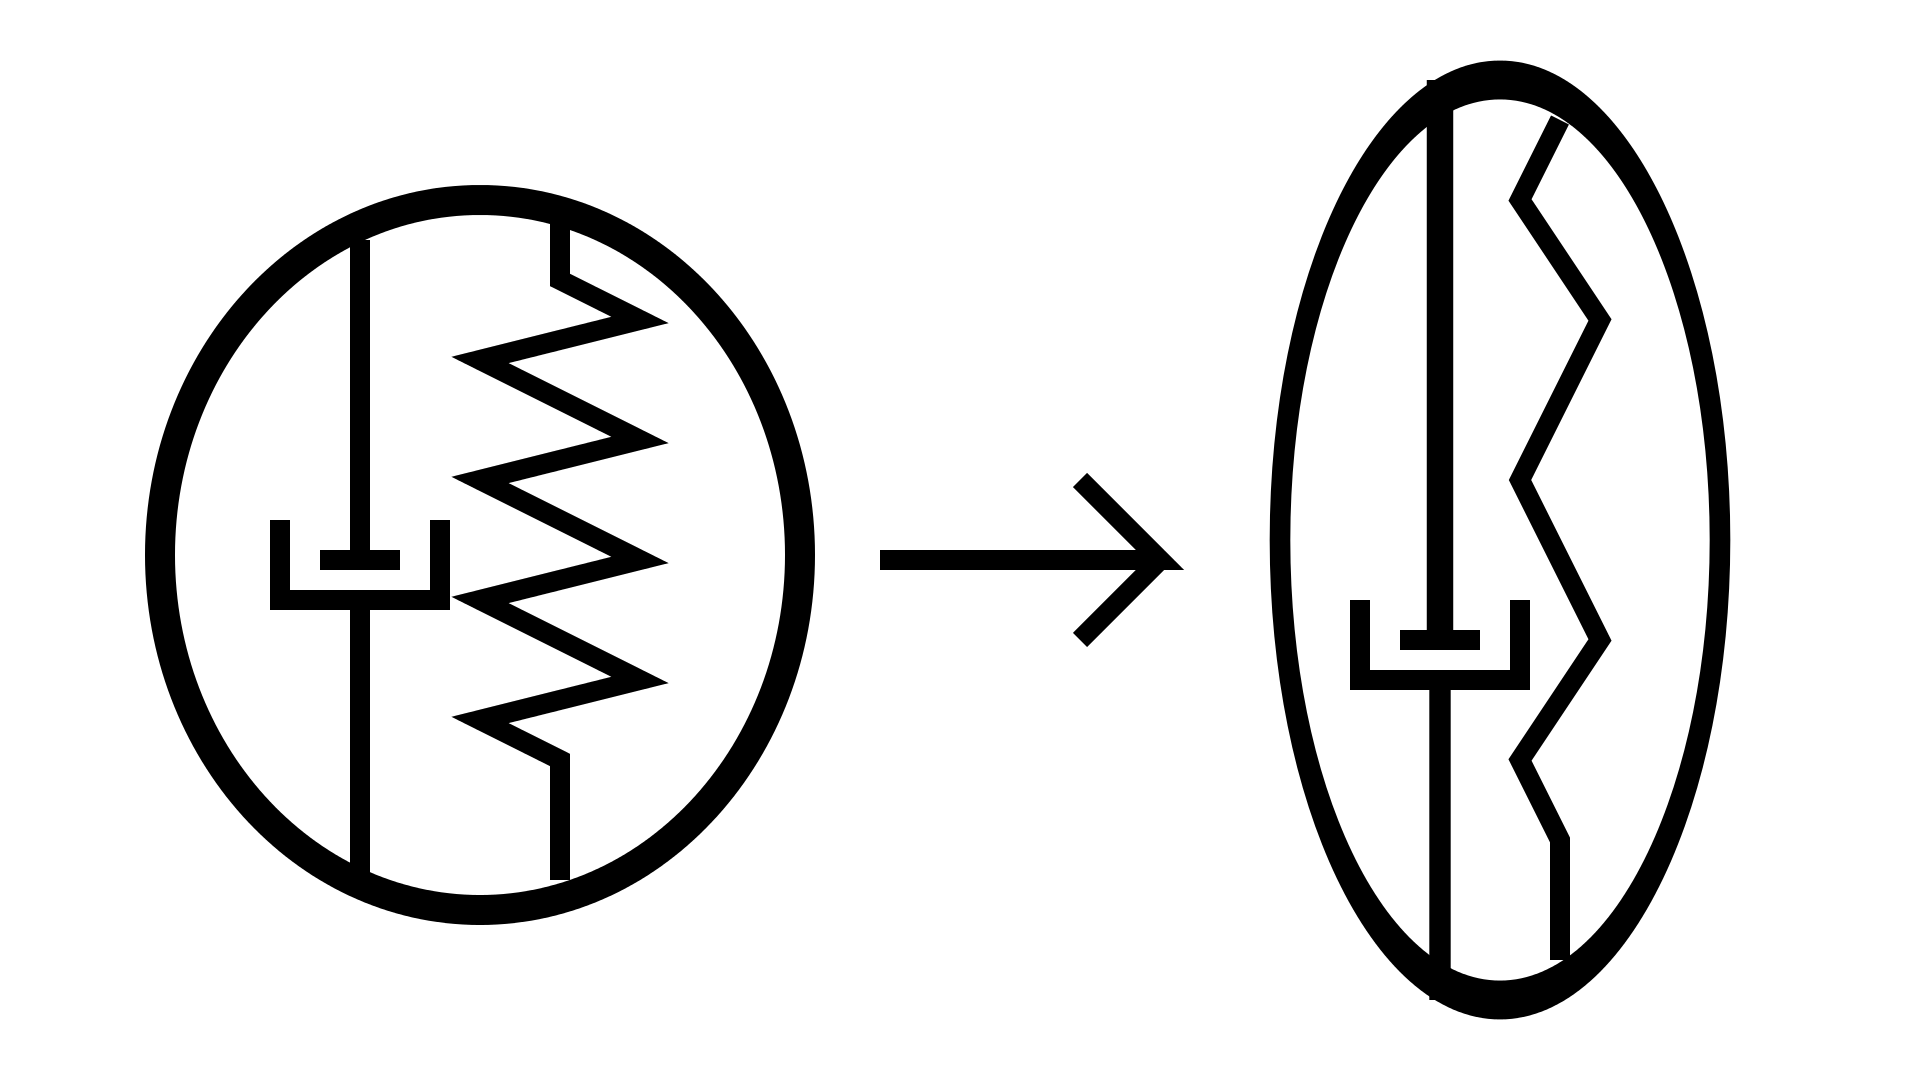
\includegraphics[width=0.8\textwidth]{TABDroplet.png}
\caption{Droplet deformation modelled by the Taylor Analogy Break-up (TAB) model.}
\end{figure} 

The equation for a spring-mass-damper system is given as follows:

\begin{equation}
\frac{d^{2}y}{dt^{2}} + 2 \zeta \omega_{0} \frac{dy}{dt} + \omega_{0}^{2}y = F(t)
\end{equation}

where $y$ is the displacement, $\zeta$ is the damping coefficient, $\omega_{0}$ is the undamped natural frequency, and $F(t)$ is a time-dependant forcing term.

For a simple droplet, the equation of motion was determined to be

\begin{equation}\label{eq:TabPde}
\frac{d^{2}y}{dt^{2}} + \frac{4C_{d}\mu}{\rho_{l}d^{2}}\frac{dy}{dt} + \frac{8C_{k}\sigma}{\rho_{l}d^{3}}y = \frac{4C_{f}\rho_{g}|\vec{v}_{rel}|^{2}}{C_{b}\rho_{l}d^{2}}
\end{equation}

where $\mu$, $d$, and $\sigma$ are the droplet viscosity, diameter and surface tension coefficient respectively and $C_{d}$, $C_{k}$, $C_{f}$ and $C_{b}$ are empirically determined constants with the following values:

\begin{subequations}
\begin{equation}
C_{d} = 10
\end{equation}
\begin{equation}
C_{k} = 8
\end{equation}
\begin{equation}
C_{f} = 2/3 \; \text{(gradual loading)}
\end{equation}
\begin{equation}
C_{f} = 1/3 \; \text{(sudden loading)}
\end{equation}
\begin{equation}
C_{b} = 1/2
\end{equation}
\end{subequations}

The value of $y$ is non-dimensional, and takes the form

\begin{equation}
y = \frac{4\Delta d_{min}}{d_{0}}
\end{equation}

where $d_{min}$ describes the deviation between the minor drop diameter and that of its original diameter, $d_{0}$.

The solution to equation \ref{eq:TabPde} has the form:

\begin{equation}\label{eq:TabPdeSolution}
y(t) = We_{c} + e^{-t/\tau_{D}}\left\{(y_{0} + We_{c})\cos{(\omega t) + \frac{1}{\omega}\left(\frac{dy_{0}}{dt} + \frac{y_{0} - We_{c}}{\tau_{D}}\right)\sin{(\omega t)}}\right\}
\end{equation}

where

\begin{equation}\label{eq:omega}
\omega = \left\{\frac{8C_{k}\sigma}{\rho_{l}d^{3}} - \frac{1}{\tau_{D}^{2}}\right\}^{\frac{1}{2}}
\end{equation}

\begin{equation}
\tau_{D} = \frac{\rho_{l}d^{2}}{2C_{d}\mu}
\end{equation}

and the critical Weber number, $We_{c}$, is

\begin{equation}
We_{c} = We\left(\frac{C_{f}}{C_{k}C_{b}}\right)
\end{equation}

When considering a single discrete time step, and assuming that the droplet initially is not deformed nor deforming ($y_{0} = \frac{dy_{0}}{dt}$ = 0), equation (\ref{eq:TabPdeSolution}) and its derivative take the forms

\begin{equation}\label{eq:TabPdeSolutionDiscretized}
y^{n+1} = We_{c} + e^{-\Delta t/\tau_{D}}\left\{(y^{n} + We_{c})\cos{(\omega \Delta t) + \frac{1}{\omega}\left(\left(\frac{dy}{dt}\right)^{n} + \frac{y^{n} - We_{c}}{\tau_{D}}\right)\sin{(\omega \Delta t)}}\right\}
\end{equation}

\begin{equation}\label{eq:TabPdeSolutionDiscretizedDeriv}
\left(\frac{dy}{dt}\right)^{n+1} = \frac{We_{c} - y^{n+1}}{\tau_{D}} + \omega e^{-\Delta t/\tau_{D}}\left\{\frac{1}{\omega}\left(\left(\frac{dy}{dt}\right)^{n} + \frac{y^{n} - We_{c}}{\tau_{D}}\right)\cos{(\omega \Delta t) - (y^{n} - We_{c})\sin{(\omega \Delta t)}}\right\}
\end{equation}

From equations (\ref{eq:TabPdeSolutionDiscretized}) and (\ref{eq:TabPdeSolutionDiscretizedDeriv}), the distortion of each droplet may be tracked. Breakup is said to occur when $y(t) \geq 1$.

After a break-up occurs, the size of the child droplets must be determined. This is done by equating the energy of the parent droplet to the combined energy of the child droplets. The energy of the parent droplet is

\begin{equation}\label{eq:Eparent}
E_{parent} = 4\pi r^{2}\sigma + K\frac{\pi}{5}\rho_{l}r^{5}\left[\left(\frac{dy}{dt}\right)^{2} + \omega^{2}y^{2}\right]
\end{equation}

where $K$ is the ratio of total energy in distortion and oscillation, and is set to

\begin{equation}
K = \frac{10}{3}
\end{equation}

The energy of the child droplets can then be shown to be

\begin{equation}\label{eq:Echild}
E_{child} = 4\pi r^{2}\sigma\frac{r}{r_{32}} + \frac{\pi}{6}\rho_{l}r^{5}\left(\frac{dy}{dt}\right)^{2}
\end{equation}

where $r_{32}$ is the Sauter mean radius of the droplet distribution. Setting $y=1$, subbing in equation (\ref{eq:omega}), and setting equations (\ref{eq:Eparent}) and (\ref{eq:Echild}) equal to each other, one obtains the equation for the Sauter mean radius as

\begin{equation}
r_{32} = \frac{r}{1 + \frac{8Ky^{2}}{20} + \frac{\rho_{l}r^{3}(dy/dt)^{2}}{\sigma}\left(\frac{6K-5}{120}\right)}
\end{equation}

The droplets can then be assumed to be normally distributed about $r_{32}$, with the number of droplets determined through mass conservation. 

The velocity of the child droplets must also be computed. A normal component of velocity is added onto the droplet, which has the form

\begin{equation}
|\vec{v}_{normal}| = C_{v}C_{b}r\left(\frac{dy}{dt}\right)
\end{equation} 

where $C_{v}$ is a constant on the order of $1$.

\section{Results}\label{sec:Results}

The following section contains results obtained from coding the evaporation and TAB droplet advection code. The code itself as been included in the appendices.

\newpage
\appendix
\section{boTAB Code - Main Module}

\begin{lstlisting}
#!/usr/bin/env python2
# -*- coding: utf-8 -*-

"""
boTAB
=====
This solver uses the popular TAB model to simulate the atomization of droplets
Author: Adam O'Brien
"""

from input import *
from math import exp, cos, sin, sqrt
from fluid import *
from evaporation import *
from TAB import *
from output import *
import copy as cp

def main():

    print ""
    print "boTAB |"
    print "-------"
    print "        Compute the break-up of a drop in a uniform cross-flow", "\n"

    # Open up a configuration file

    userInput = readInputFile()

    freestream = Freestream()
    initialDroplet = Droplet()
    dropletInlet = DropletInlet()

    # Set object parameters from the input file

    setObjectParametersFromInput(userInput, freestream, initialDroplet, dropletInlet)

    # Set-up the simulation parameters in accordance with the input

    maxTime = userInput["maxTime"]
    nTimeSteps = userInput["nTimeSteps"]

    # Initialize a droplet list, with one copy of the initial droplet

    droplets = [cp.deepcopy(initialDroplet)]

    # Initialize misc parameters

    dt = maxTime/nTimeSteps
    t = [0.]
    nChildDroplets = 0

    # Begin the simulation

    print "\nBeginning time-stepping..."

    ###########################################
    #                                         #
    #           Main Iteration Loop           #
    #                                         #
    ###########################################

    for stepNo in range(1, nTimeSteps + 1):

        for droplet in droplets:

            droplet.advectPredictorCorrector(freestream, dt)

        evaporate(freestream, droplets, dt)
        nChildDroplets += breakupTab(freestream, droplets, dt)

        dropletInlet.addDrops(initialDroplet, droplets, dt)
        t.append(t[-1] + dt)

        if stepNo%(nTimeSteps/20) == 0:

            completionPercentage = float(stepNo)/float(nTimeSteps)*100.

            print "-----------------------------------------------------------"
            print "Time-stepping completion     : %s%%"%(completionPercentage)
            print "Number of droplets in domain :", len(droplets)
            print "Simulation time elapsed      : %s seconds"%(t[-1])
            print "Simulation time remaining    : %s seconds"%(maxTime - t[-1])
            print "Number of child drops        :", nChildDroplets

    print "\nTime-stepping complete. Finalizing output..."

    plotDroplets(droplets)

# Execute the main function

if __name__ == "__main__":
    main()
\end{lstlisting}
\newpage
\section{boTAB Code - Fluid Module}

\begin{lstlisting}

#/usr/bin/env python2
# -*- coding: utf-8 -*-

"""
boTAB
=====
This module contains classes and function for the modelling of droplets in
freestream flows
Author: Adam O'Brien
"""

from math import sqrt, pi, exp
import copy as cp
import random

# Vector class for position/velocity

class Vector(object):

    def __init__(self, x, y):
        self.x = x
        self.y = y

    def __repr__(self):

        return "%s, %s"%(self.x, self.y)

    def __add__(self, other):

        return Vector(self.x + other.x, self.y + other.y)

    def __sub__(self, other):

        return Vector(self.x - other.x, self.y - other.y)

    def __mul__(self, other):

        return Vector(self.x*other, self.y*other)

    def mag(self):
        return sqrt(self.x**2 + self.y**2)

    def normalVector(self):
        return Vector(self.y, -self.x)

    def scale(self, other):
        return Vector(self.x*other, self.y*other)

    def rVector(self, other):

        return other - self

    def unitVector(self):

        return self.scale(1./self.mag())

def dot(u, v):

    return u.x*v.x + u.y*v.y

# Freestream class for representing the freestream flow

class Freestream(object):

    def __init__(self, velocity = Vector(40., 0.), gravity = Vector(0., 0.)):

        # constructed properties

        self.velocity = velocity
        self.gravity = gravity

        # default air proplerties (can be changed)

        self.mu = 18.27e-6
        self.Pambient = 101325.
        self.Tambient = 800.
        self.Cp = 1.0005
        self.k = 0.0257
        self.M = 28.97
        self.Pr = self.Cp*self.mu/self.k

        # Computed properties

        self.rho = self.Pambient/(286.9*self.Tambient)

# Droplet class for representing droplets

class Droplet(object):

    def __init__(self, radius = 5e-4, position = Vector(0., 0.), velocity = Vector(0., 10.)):

        # constructed properties

        self.radius = radius
        self.position = position
        self.velocity = velocity

        # default water properties (can be changed)

        self.rho = 998.
        self.mu = 8.94e-4
        self.sigma = 0.07262
        self.Tboil = 373.
        self.Tcrit = 647.096
        self.T = 400.
        self.L = 2257.
        self.Cp = 4.183
        self.k = 0.58
        self.M = 18.01528

        # TAB properties

        self.y = 0.
        self.dydt = 0.

    def __repr__(self):

        return "Radius: %s\nPosition: %s\nVelocity: %s"%(str(self.radius), \
        self.position, self.velocity)

    def diameter(self):

        return 2.*self.radius

    def volume(self):

        return (4./3.)*pi*self.radius**3

    def area(self):

        return pi*self.radius**2

    def mass(self):

        return self.volume()*self.rho

    def Pvap(self, freestream):

        Tref = (2./3.)*self.T + (1./3.)*freestream.Tambient

        a1 = -7.85951783
        a2 = 1.84408259
        a3 = -11.7866497
        a4 = 22.6807411
        a5 = -15.9618719
        a6 = 1.80122502

        tau = 1. - Tref/self.Tcrit

        pOverPc = exp((a1*tau + a2*tau**1.5 + a3*tau**3 + a4*tau**3.5 + a5*tau**4 + a6*tau**7.5)*self.Tcrit/self.T)

        return pOverPc*22064.

    def We(self, freestream):

        vRel = self.velocity.rVector(freestream.velocity)

        return freestream.rho*dot(vRel, vRel)*self.radius/self.sigma

    def Re(self, freestream):

        return freestream.rho*(freestream.velocity - self.velocity).mag()*self.diameter()/freestream.mu

    def dragCoefficient(self, freestream):

        # This drag coefficient for a sphere is based on the correlation of
        # F.A. Morrison in "An Introduction to Fluid Mechanics"

        Re = self.Re(freestream)

        return 24./Re + 2.6*(Re/5.)/(1. + (Re/5.)**1.52) + 0.411*(Re/263000.)**-7.94/(1. + (Re/263000.)**-8.) + (Re**0.8/461000.)

    def dragForce(self, freestream):

        Cd = self.dragCoefficient(freestream)

        vRel = freestream.velocity - self.velocity

        return vRel.unitVector()*0.5*freestream.rho*dot(vRel, vRel)*Cd*self.area()

    def acceleration(self, freestream):

        return self.dragForce(freestream).scale(1./self.mass()) + freestream.gravity

    def advectEuler(self, freestream, dt):

        a = self.acceleration(freestream)

        self.position += self.velocity*dt + a*0.5*dt**2
        self.velocity += a*dt

    def advectPredictorCorrector(self, freestream, dt):

        originalPosition = self.position

        a = self.acceleration(freestream)
        f1 = self.velocity + a*0.5*dt

        self.position += f1*dt

        a = self.acceleration(freestream)
        f2 = self.velocity + a*0.5*dt

        self.position = originalPosition + (f1 + f2)*0.5*dt
        self.velocity += a*dt

    def printAll(self):

        print "Radius:", self.radius
        print "Rho:", self.rho
        print "mu:", self.mu
        print "sigma:", self.sigma
        print "Boiling Temp:", self.boilingTemp
        print "Latent Heat:", self.latentHeat
        print "Specific Heat:", self.specificHeat
        print "k:", self.k
        print "Position:", self.position
        print "Velocity:", self.velocity

class DropletInlet(object):

    def __init__(self, newDropletFrequency = 1000, inletWidth = 0.005, velocityDeviation = 0.):

        self.newDropletFrequency = newDropletFrequency
        self.inletWidth = inletWidth
        self.velocityDeviation = velocityDeviation
        self.timeSinceLastDroplet = 0.
        self.newDropletPeriod = 1./self.newDropletFrequency
        self.dropsAdded = 0

    def addDrops(self, initialDroplet, droplets, dt):

        self.timeSinceLastDroplet += dt

        nDropsToAdd = int(self.timeSinceLastDroplet/self.newDropletPeriod)
        self.timeSinceLastDroplet -= float(nDropsToAdd)*self.newDropletPeriod

        if nDropsToAdd > 0:
            self.dropsAdded += nDropsToAdd

        for i in range(0, nDropsToAdd):

            droplets.append(cp.deepcopy(initialDroplet))
            droplets[-1].position.x += random.uniform(-0.5*self.inletWidth, 0.5*self.inletWidth)
            droplets[-1].velocity.x += random.normalvariate(0., self.velocityDeviation.x)
            droplets[-1].velocity.y += random.normalvariate(0., self.velocityDeviation.y)
            
\end{lstlisting}

\newpage
\section{boTAB Code - Input Module}

\begin{lstlisting}

# -*- coding: utf-8 -*-

"""
boTAB
=====
This module is for simple file input and configuration
Author: Adam O'Brien
"""

from fluid import Vector

def str2num(string):

    if string.partition("/")[1] == "/":

        string = string.partition("/")

        return float(string[0])/float(string[2])

    elif string.partition(",")[1] == ",":

        string = string.partition(",")

        return Vector(float(string[0]), float(string[2]))

    else:

        try:

            return int(string)

        except ValueError:

            return float(string)


def process(inputDict, line):

    line = line.replace("\n", "")
    line = line.replace(" ", "")
    line = line.partition("#")
    line = line[0]

    if line == "":
        return

    line = line.partition("=")

    if not line[1] == "=":
        print "Warnining, potentially bad input:", line

    inputDict[line[0]] = str2num(line[2])

    return

def readInputFile(filename = "config.in"):

    userInput = {}

    print "Reading from input file \"config.in\"..."

    with open(filename) as inFile:

        for line in inFile:

            process(userInput, line)

    print "The following input parameters have been loaded from \"{}\"".format(filename), "\n"

    for parameter in userInput:

        print parameter, "=", userInput[parameter]

    print "Finished reading from input file \"config.in\"."

    return userInput

def setObjectParametersFromInput(userInput, freestream, droplet, inlet):

    # Freestrean properties

    freestream.rho = userInput["freestreamRho"]
    freestream.mu = userInput["freestreamMu"]
    freestream.Tambient = userInput["freestreamTambient"]
    freestream.Cp = userInput["freestreamCp"]
    freestream.K = userInput["freestreamK"]
    freestream.velocity = userInput["freestreamVelocity"]
    freestream.gravity = userInput["freestreamGravity"]
    freestream.M = userInput["freestreamM"]

    # Initial droplet properties

    droplet.radius = userInput["dropletRadius"]
    droplet.rho = userInput["dropletRho"]
    droplet.mu = userInput["dropletMu"]
    droplet.sigma = userInput["dropletSigma"]
    droplet.Tboil = userInput["dropletTboil"]
    droplet.L = userInput["dropletL"]
    droplet.Cp = userInput["dropletCp"]
    droplet.K = userInput["dropletK"]
    droplet.position = userInput["dropletPosition"]
    droplet.velocity = userInput["dropletVelocity"]
    droplet.M = userInput["dropletM"]

    # Droplet inlet properties

    inlet.newDropletFrequency = userInput["inletDropletCreationFrequency"]
    inlet.inletWidth = userInput["inletWidth"]
    inlet.velocityDeviation = userInput["inletVelocityDeviation"]

\end{lstlisting}

\newpage
\section{boTAB Code - Output Module}

\begin{lstlisting}

# -*- coding: utf-8 -*-

"""
boTAB
=====
This module is for various plotting outputs
Author: Adam O'Brien
"""

import matplotlib.pyplot as plt
import matplotlib.animation as animation

def plotDroplets(droplets):

    xcoords = [droplet.position.x for droplet in droplets]
    ycoords = [droplet.position.y for droplet in droplets]
    radii = [50000.*droplet.radius for droplet in droplets]

    plt.axis('equal')
    plt.grid(True)
    plt.xlabel('x (m)', fontsize=16)
    plt.ylabel('y (m)', fontsize=16)

    plt.scatter(xcoords, ycoords, s=radii, alpha=0.5)

    plt.show()
    
\end{lstlisting}

\newpage
\section{boTAB Code - Evaporation Module}

\begin{lstlisting}

# -*- coding: utf-8 -*-

"""
boTAB
=====
This module contains classes and function for the modelling of droplet
evaporation in freestream flows
Author: Adam O'Brien
"""

from math import log, sqrt, fabs, pi

def clausiusClapeyron(freestream, droplet):

    # This function determines the water vapour mass fraction at the surface
    # of a droplet

    return 1./(1. + freestream.Pambient*freestream.M/((droplet.Pvap(freestream) - 1.)*droplet.M))

def evaporate(freestream, droplets, dt):

    for i in range(0, len(droplets)):

        Yls = clausiusClapeyron(freestream, droplets[i])

        BM = Yls/(1. - Yls)

        Re = droplets[i].Re(freestream)
        Pr = freestream.Pr

        gamma = 8.*freestream.k*log(1. + BM)/(freestream.Cp*droplets[i].rho)*(1. + 0.3*Re**0.5*Pr**(1./3.))

        D2 = droplets[i].diameter()**2 - gamma*dt

        if D2 > 0.:

            droplets[i].radius = 0.5*D2**0.5

        else:

            droplets[i].radius = 0.

    # Discard any droplets that have a radius less than the tolerance, ie they
    # are completely evaporated

    droplets[:] = [droplet for droplet in droplets if not droplet.radius <= 1e-10]

\end{lstlisting}

\newpage
\section{boTAB Code - TAB Module}

\begin{lstlisting}

# -*- coding: utf-8 -*-

"""
boTAB
=====
This module contains the functions necessary for TAB breakup
Author: Adam O'Brien
"""

from math import exp, sin, cos, fabs
import numpy as np
import copy as cp
from fluid import *

# Model constants

Cb = 0.5
Ck = 8.
Cd = 5.
Cf = 1./3.
Cd = 5.
K = 10./3.
Cv = 1.

def getSMR(droplet):

    # This function computes the Sauter Mean Radius (SMR) of the child droplets after a break-up

    rOverRmean = 1. + (K/5.)*Ck*Cb**2 + droplet.rho*droplet.radius**3/droplet.sigma*Cb**2*droplet.dydt**2*(6.*K - 5.)/30.

    return droplet.radius/rOverRmean

def breakupTab(freestream, droplets, dt):

    newDroplets = []

    for droplet in droplets:

        Wec = droplet.We(freestream)*Cf/(Ck*Cb)
        td = droplet.rho*droplet.diameter()**2/(2.*Cd*droplet.mu)
        omega = (8.*Ck*droplet.sigma/(droplet.rho*droplet.diameter()**3) - (1./td**2))**0.5

        yn = droplet.y

        droplet.y = Wec + exp(-dt/td)* \
                    ((yn - Wec)*cos(omega*dt) + 1./omega*(droplet.dydt + (yn - Wec)/td)*sin(omega*dt))

        droplet.dydt = (Wec - droplet.y)/td + \
                       omega*exp(-dt/td)* \
                       (1./omega*(droplet.dydt + (yn - Wec)/td)*cos(omega*dt) - (yn - Wec)*sin(omega*dt))

        if droplet.y >= 1.:

            rSmr = getSMR(droplet)

            # Begin sampling droplets

            volOfNewDrops = 0.

            while True:
                
                newRadius = np.random.normal(rSmr, 0.2*rSmr)
                
                if newRadius < 0.:
                    
                    continue
                
                randomNo = np.random.uniform(-1, 1)                
                
                newVelocity = droplet.velocity + droplet.velocity.normalVector().unitVector()*Cb*droplet.radius*droplet.dydt*(randomNo/fabs(randomNo))                
                
                newDroplet = Droplet(newRadius, cp.copy(droplet.position), cp.copy(newVelocity))
                
                newDroplets.append(newDroplet)
                
                volOfNewDrops += newDroplets[-1].volume()
                
                if volOfNewDrops >= droplet.volume():
                    
                    break
                
    # Remove the old parent droplets
                
    droplets[:] = [droplet for droplet in droplets if droplet.y < 1.]
    
    # Add the newly created child droplets
    
    for droplet in newDroplets:
        
        droplets.append(cp.deepcopy(droplet))
        
    # Return the number of droplets created
        
    return len(newDroplets)

\end{lstlisting}

\end{document}
